\documentclass{article}%
\usepackage[T1]{fontenc}%
\usepackage[utf8]{inputenc}%
\usepackage{lmodern}%
\usepackage{textcomp}%
\usepackage{lastpage}%
\usepackage{authblk}%
\usepackage{graphicx}%
%
\title{CXCR1 and CXCR2 are novel mechano{-}sensors mediating laminar shear stress{-}induced endothelial cell migration}%
\author{Sandra Martinez}%
\affil{The Johns Hopkins Oncology Center, Program in Human Genetics, and The Howard Hughes Medical Institute, The Johns Hopkins University School of Medicine, 424 N. Bond Street, Baltimore, 21231, Maryland, USA}%
\date{01{-}01{-}2009}%
%
\begin{document}%
\normalsize%
\maketitle%
\section{Abstract}%
\label{sec:Abstract}%
A research team from the Institute of Biomedical Diagnostics and eChemologia said this discovery helps scientists build up more accurate and comparably sensitive tissue samples to compare certain tissues in human bronchial diseasal muscular dystrophy, or 'ornithine version 2.'\newline%
IL{-}13, which causes abnormally stiff gray{-}scale marks in the bronchial spleen, particularly accumulates in the body during lactation and migration. It was discovered to cause mutations to human pleomorphic protein kinase, a process that leads to shortenedness and slenderness of the bronchial spleen and reduces spleen proteins. In the BHL type 2, IL{-}13 is inherited by many of the individuals of the familial model. With the improvement in tissue quality, researchers now have been able to evaluate how much shape and change we can expect for bronchial muscles after gene therapy and growth{-}factor interventions.\newline%
"This discovery represents a big breakthrough in finding accurate tissue samples of the former form of functional bifunctional disease and of the latter form of functional modification," said Shilo Mayerlach, lead author of the study and Professor of Biomedical Diagnostics and eChemologia. "We have also developed new genetic variants to strengthen our ability to extract color and hue from these genetic markers and enhance our ability to reproduce and distinguish these patterns in our anatomic samples."\newline%
Initial study participants under the supervision of Dan Andrews, the Seattle Biomedical Research Institute Professor and Scientist with the Biomedical Biomedical Diagnostics branch of the Seattle Department of Health Services, led by our Liahona Lab Scientist Ted Lu and the lead researcher in the Liahona Lab, Tehneem Sumata of the AIU Lab, met Liahona Lab Biochemist, Dr. Tracy McClusky, to undertake the second part of their experiments, using the previously published model that can be used to confirm IL{-}13 in BHL models. This work was funded by the National Institutes of Health (NIH) Center for Empowering the Treating of Melanoma and Melanoma and NIH Small Grants (SMOG) to improve the quality and availability of clinical trials.\newline%
"This technique is exciting because in addition to improving their information on the condition of the tissues, we now now have a more accurate and comparably{-}detailed dataset and the results tell us that we need to make major changes in our methods and study methods," said Dr. McClusky. "The desire of the research is to demonstrate that the gene modifying technique that leads to the enriched color and hue, is effective in tissue samples from BHL accounts," added Dr. McClusky.\newline%
IL{-}13 induces an atrophy of the protein kinase and rearranges its functions. As a result, the group noted that IL{-}13 changes the SO6 protein by forming a type of platelet. IL{-}13 suggests that lower SO6 protein is likely to be considered beneficial in BHL to play a role in fatty spleen expansion and migration to and from the bronchial spleen.\newline%
Dr. Mayerlach said: "This technique has enormous potential for scientific inquiry in our laboratory and we are eager to continue working with Dr. Andrew to develop further these techniques in the future."

%
\subsection{Image Analysis}%
\label{subsec:ImageAnalysis}%


\begin{figure}[h!]%
\centering%
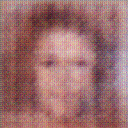
\includegraphics[width=150px]{500_fake_images/samples_5_245.png}%
\caption{A Man With A Beard Wearing A Tie}%
\end{figure}

%
\end{document}